\documentclass[tikz, border=1pt]{standalone}

\usepackage{xcolor}
\usetikzlibrary{arrows.meta}
\begin{document}
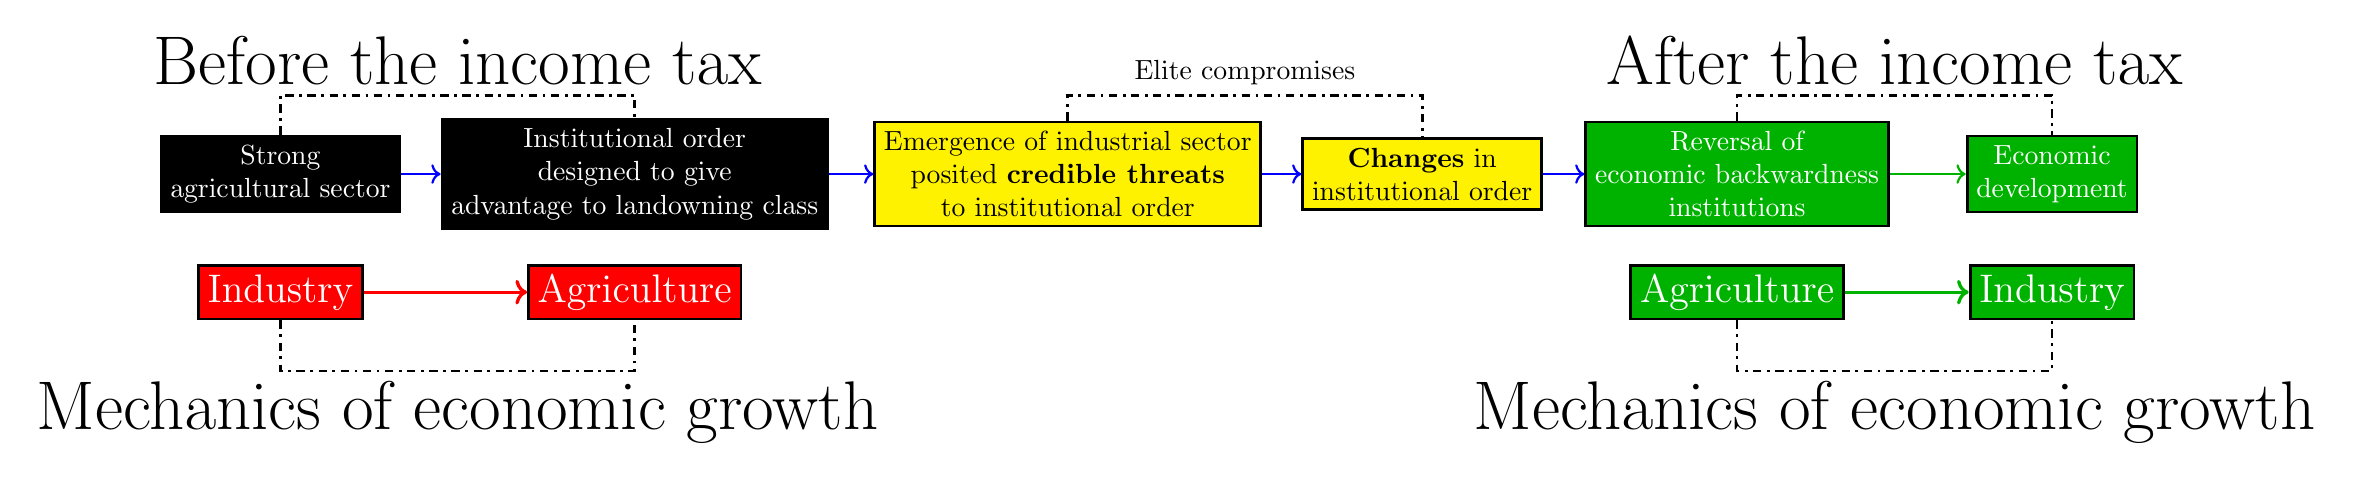
\begin{tikzpicture}[line width=1pt]


% 1










% 2
\node[draw,align=center,fill=black,text=white] (ArgumentA2) at (1,1) {Strong\\agricultural sector};

\node[draw,align=center,fill=red,text=white] (ArgumentA2b) at (1,-0.5) {{\Large Industry}};
\node[draw,align=center,fill=red,text=white] (ArgumentA3b) at (5.5,-0.5) {{\Large Agriculture}};


\node[draw,align=center,fill=black,text=white] (ArgumentB2) at (5.5,1) {Institutional order\\designed to give\\advantage to landowning class};
\node[draw,align=center,fill=yellow,text=black] (ArgumentC) at (11,1) {Emergence of industrial sector\\posited {\bf credible threats}\\to institutional order};
\node[draw,align=center,fill=yellow,text=black] (ArgumentD2) at (15.5,1) {{\bf Changes} in\\institutional order};


\draw[dash dot] (ArgumentA2b) -- ++(0,-1) -| (ArgumentA3b)
node[below, near start] {{\Huge Mechanics of economic growth}}; % HERE


%\node[draw,align=center] (ArgumentD23) at (8,4) {Failure to incorporate\\both elites}; 

%\node[draw,fill=red,text=white] (ArgumentE2) at (20.5,1) {Failed state};

\node[draw,fill=black!30!green,text=white,align=center] (ArgumentA4) at (19.5,1) {Reversal of\\economic backwardness\\institutions};
\node[draw,fill=black!30!green,text=white,align=center] (ArgumentB4) at (23.5,1) {Economic\\development};


\node[draw,align=center,fill=black!30!green,text=white] (ArgumentA2c) at (19.5,-0.5) {{\Large Agriculture}};
\node[draw,align=center,fill=black!30!green,text=white] (ArgumentA3c) at (23.5,-0.5) {{\Large Industry}};


\draw[<-,draw=black!30!green,thick] (ArgumentB4) to (ArgumentA4);
\draw[->,draw=red,very thick] (ArgumentA2b) to (ArgumentA3b);
\draw[->,draw=black!30!green,very thick] (ArgumentA2c) to (ArgumentA3c);



\draw[->,draw=blue,thick] (ArgumentD2) to (ArgumentA4);
%\draw[|-|,draw=blue,thick] (ArgumentC) to (ArgumentD23);

%\draw[->,draw=blue,thick] (ArgumentB4) to (ArgumentE2);




\draw[->,draw=blue,thick] (ArgumentB2) to (ArgumentC);
\draw[<-,draw=blue,thick] (ArgumentD2) to (ArgumentC);
\draw[->,draw=blue,thick] (ArgumentA2) to (ArgumentB2);

\draw[dash dot] (ArgumentA2) -- ++(0,1) -| (ArgumentB2)
node[above, near start] {{\Huge Before the income tax}};


\draw[dash dot] (ArgumentA2c) -- ++(0,-1) -| (ArgumentA3c)
node[below, near start] {{\Huge Mechanics of economic growth}};

\draw[dash dot] (ArgumentC) -- ++(0,1) -| (ArgumentD2) node[above, near start] {Elite compromises}; % here


\draw[dash dot] (ArgumentA4) -- ++(0,1) -| (ArgumentB4) node[above, near start] {{\Huge After the income tax}}; % here






\node at (6., -1.0) {};






%%%








  
\end{tikzpicture}
\end{document}